%!TEX root = /Users/Ken/Dropbox/Master's Thesis/Paper/my thesis/main.tex
\chapter{Evaluation}
\label{chapter:evaluation}

\section{Reference Scenario}
We planned to build an IoT service with web technology that differed from the pervious solution, database-centric approach, which largely relies on Ajax for data exchange. 

The prevision of the thesis was constructed in two parts: web technology and IoT; Its solution should integrate the two parts into a coherent service. Following the consideration of HTML5 connectivity features, we focused on the WebSocket protocol which fills the part of web technology. As for IoT, which covers a wide area, we selected one scenario -- smart lighting control -- with a sensor and an actuator from many IoT visions such as NFC applications, smart housing and phones connectivity. 

Compared with other HTML5 communication technologies, the WebSocket protocol is more mature, having ready made auxiliary libraries with a feasible amount of selections. The WebSocket protocol, additionally, supports subprotocols where WAMP fills the blank and provides the messaging patterns which furthermore covers the two most important interaction in IoT service.

The Sensor and actuator are two of the most common ``things'' in IoT architecture. The sensor collects data, while the actuator emits commands. We evaluated these two components matches the web technology, WebSockets with WAMP. We, further, collected several IoT scenario assumptions - high lever descriptions of what we thought might work. For example, we drafted using sensors in a phone, collected data and reported to data centre; Applying a searching function in the real world; or smart building. We evaluated the phone case is a bit far away from web technology and the implementation might involve more mobile technology rather than web technology. As for the searching function, it might involve more hardware configurations and physical experiments. 

Among of all, thus, we trimmed down the assumptions and focused on the smart building scenario. We proposed several hypotheses -- more granular descriptions of the assumption -- which target on the following specific areas: sensor deployment, data collection, data transmission, endpoint visualisation and others, such as business model level cases. Moreover, we continuously decreased the amount of areas to work on. Data transmission is related to the thesis scope where it matches Pub/Sub and RPC patterns; While endpoints visualisation provides a human friendly interface to review data, and it, besides, performs simulation, such as, simulating the environment.

Finally, we started to experiment on the smart lighting and control application, an IoT service about a sensor and an actuator with the WebSocket. 

\section{Tools and Setup}
Before we started the thesis project, we assumed the front-end environment would largely rely on web browsers. As a result, we expected to build it with JavaScript. For this reason, we found AutobahnJS\footnote{http://autobahn.ws/js}, an open source JavaScript networking library. 

AutobahnJS supports WAMP at a higher level, while supports the WebSocket protocol at lower level. Thus, it is feasible to create a real-time enabled HTML5 applications with the library. Moreover, AutobahnJS has - another advantage of AutobahnJS - clear tutorials and documents.

As for the backend deployment, it relatively has more options where a list of existing library has been being appended to support WAMP. From the perspective of programming languages, there are implementation on Python, PHP, JavaScript, Java and others. Our implementation is based on WAMP.IO, a NodeJS library supporting WAMP. WAMP.IO does not handle the WebSocket protocol, but its dependency does. 

At the beginning, there were some technical problems in WAMP.IO, leading an initial connection failure with a WAMP client. Thus, we moved to Ratchet, a backend implementation using PHP, until the developer fixed those problems. Compared WAMP.IO with Ratchet, we found out Ratchet is more verbose, from the perspective of development: there are some features we did not need. WAMP.IO, however, targets the desired features - Pub/Sub and RPC - straightforward. With its simple architecture, we could easily customise the library to match demands more closely. Moreover, its developer, behind the library, actively identified and fixed bugs, making the whole development reliable. 

\section{Simulation}
We mentioned about the light, the switch/dimmer, the sensor and the sun in the thesis. Considering the thesis scope, we decided to focus on the software level, rather than the hardware part. Thus, we, at the current stage, simulated the light, the switch, the sensor and the sun. 

For the simulation, we ported the most relevant features -- directly related to the implementation -- to the software level. Meanwhile, we analysed its possibility bringing those features and the results back to physical objects. 

For example, a light bulb emits light, where the light is the key link connecting the virtuality to the reality. We mapped light luminance into digital numbers at the software level. The luminance can thus be controlled by adjusting digital numbers. The light status -- on and off -- similarly, can be simulated by e.g. boolean value. 

As for the switch/dimmer, a switch turns on or off the light, while a dimmer adjusts the luminance of the light at a certain range. The action of turning/adjusting is the key part that we simulated. The simulation of turning/adjusting, is, being the case, to connect the light component and the switch/dimmer component at the software level, and making the light response to the action of the switch/dimmer. This is, actually, how a switch/dimmer does in the real world.

A sensor, generally, converts physical quantity into digital signal which can be further read or analysed by a observer or an instrument. Thus, a sensor is, essentially, a programme that provides data at the software level. Consequently, we simulated the sensor through a programme piping the output of the sun to the light.

As for the sun, we also ported it to the software level. To do so, we made a programme that generated a sequence of numbers periodically increasing to a peak then recurring.

\section{Measurements}
We measured about overheads and Roundtrip Delayed Time (RTT) comparing WAMP with MQTT. Figure \ref{fig:overhead} illustrates the message overheads on WAMP and MQTT.

\begin{figure}[t]
  \begin{center}
    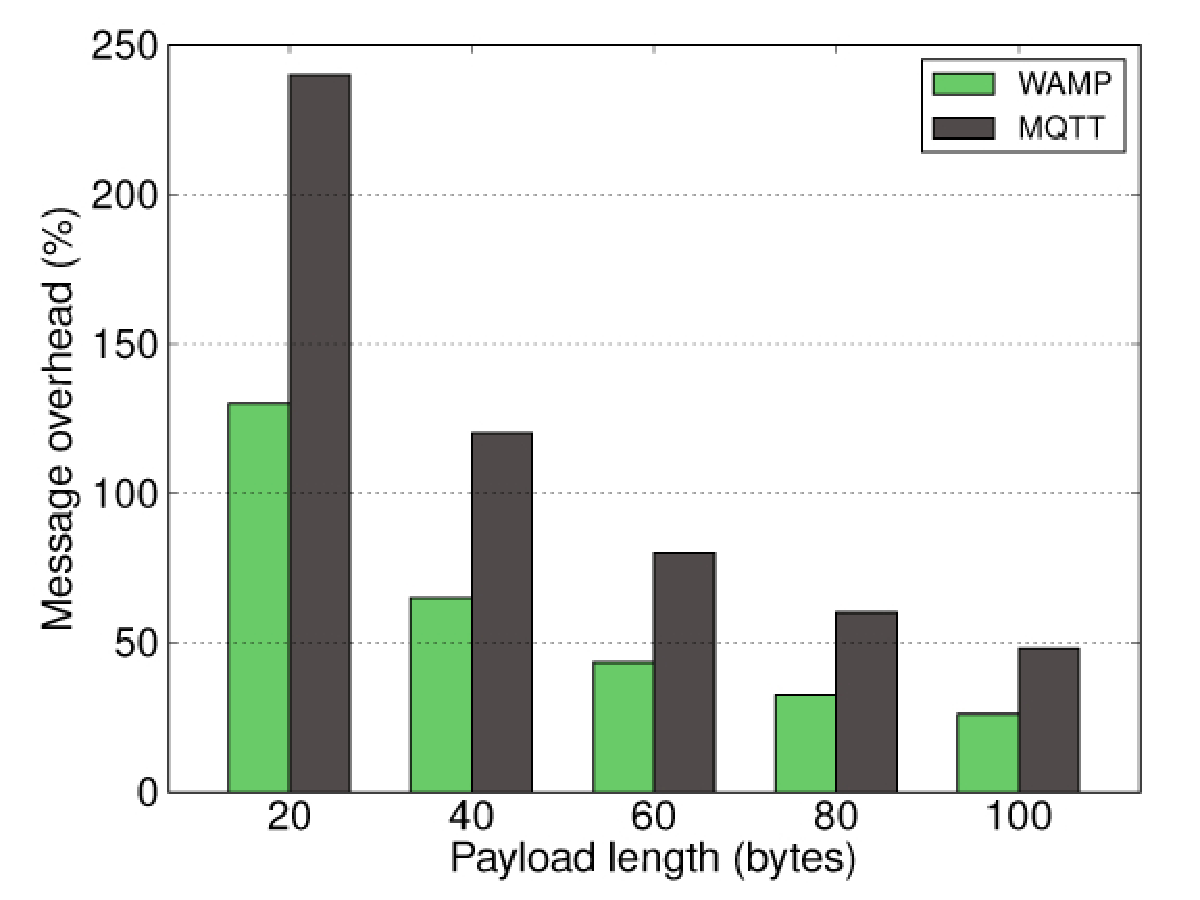
\includegraphics[width=0.7\textwidth]{images/overhead.pdf}
    \caption{Message Overhead}
    \label{fig:overhead}
  \end{center}
\end{figure}

WAMP shows its lightweight design better than that of MQTT. For each 20 bytes of data sent, WAMP will have 1.25 times overheads larger than the message itself, while MQTT will have around 2.4 times overheads generated. 

Figure \ref{fig:rtt} illustrates the message RTT on WAMP and MQTT.

\begin{figure}[t]
  \begin{center}
    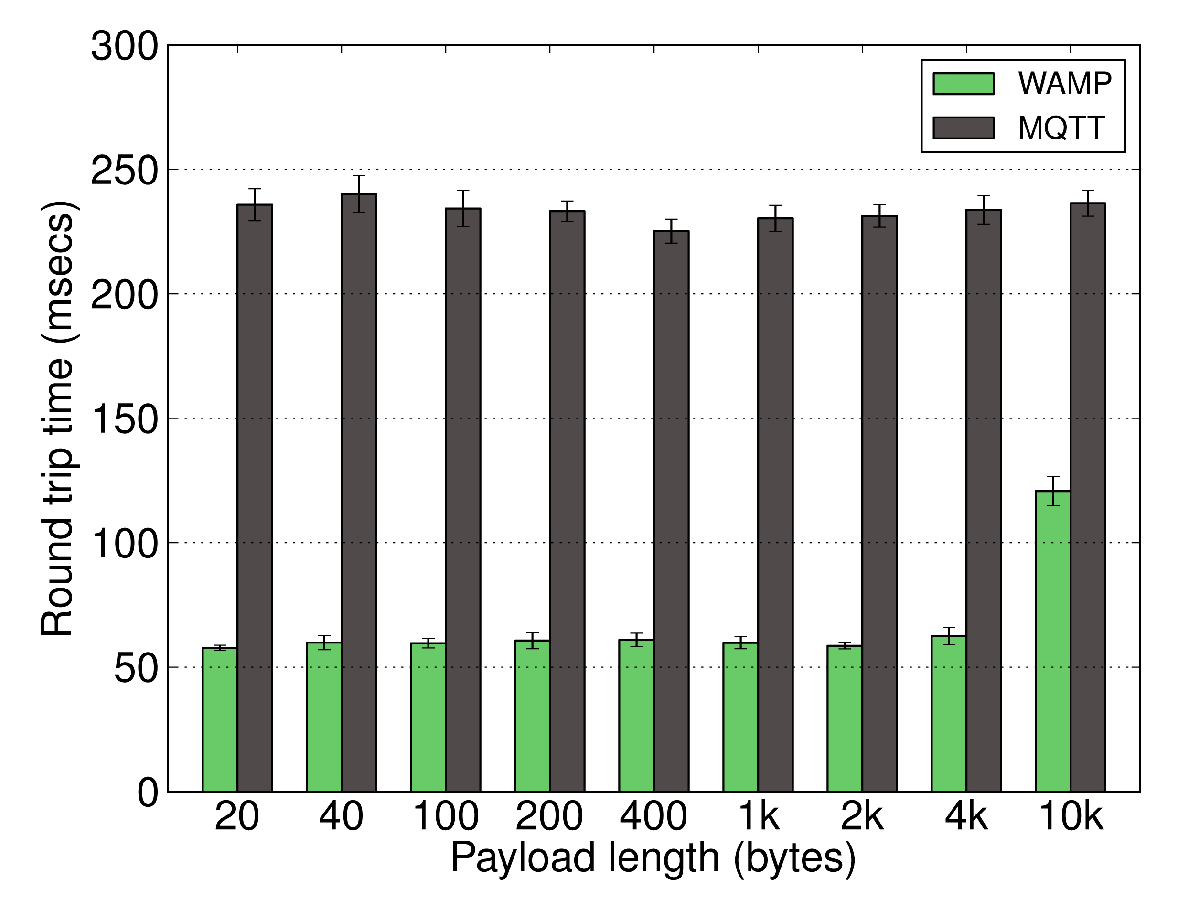
\includegraphics[width=0.7\textwidth]{images/rtt.pdf}
    \caption{Message RTT}
    \label{fig:rtt}
  \end{center}
\end{figure}

We measured the RTT from a local workstation to an Amazon micro instance in Ireland. And the result we got is, generally, MQTT has a longer RTT than that of WAMP; WAMP RTT starts to increase after sending 10k bytes, while MQTT stays constantly. The sudden increment could be caused by the programme design, the workstation or the Amazon instance we used. As the package size increased, the processing and queueing time might consequently enlarge. 

\section{Scalability}
In Pub/Sub and RPC Patterns for web-based IoT applications, the broker(s) plays a key role managing the interconnection of clients. Each client differs from others by its ID. Thus, the nature of scaling in these patterns is the implementation of addressing clients. Further communications and interactions, among users and backends, rely on the successful navigation of the broker(s).

In the scenario of the smart lighting and controlling application, the scaling issue generated by the enlarging amount of lights, switches and light sensors. Considering the limited resources that an embedded web server are assigned, the architecture might not suit for a large scale without other resources support such as extra brokers with power sources.

As for the database-centric pattern, the CouchDB solution naturally provides a reliable and flexible way to scale horizontally and to replicate, with the growing amount of data. The database acts as a hub between IoT devices and end users, while it can be further developed into cloud-based architecture which maximises its scalability. 

\section{Security}
The WebSocket protocol supports connections over Transport Layer Security (TLS). TSL provides communications security over the Internet \cite{dierks2008rfc}. Furthermore, the WebSocket protocol providers applicable security considerations as the followings \cite{rfc64552012web}: 

\begin{itemize}
% You can use this command to set the items in the list closer to each other
% (ITEM SEParation, the vertical space between the list items) 
\setlength{\itemsep}{0pt}
\item \emph{Non-browser} Client resistant. The WebSocket protocol prevents malicious running inside a web browser. 
\item \emph{Origin Considerations}. The WebSocket protocol provides a way for servers that do not intend to process input from web pages from other origins.
\item \emph{Masking}. All data from clients to servers are masked, so that the attacker does not have knowledge about how the data being sent.
\end{itemize}

The security considerations on database-centric pattern implemented by CouchDB has been discussed in \cite{francesco2012storage}. As for database, one of the most important security issue is authentication and access control. It is notable that CouchDB, by default, does not turn on access control for different users. This means, everybody has the same permission as the administrator. CouchDB authenticates users in many ways, such as HTTP basic authentication, cookie authentication and OAuth \cite{hammer2010oauth}. CouchDB has started to support Secure Sockets Layer (SSL) since CouchDB version 1.1, and thus provides communication security over the Internet.
